\section{Background}\label{sec:background}
\subsection{Large Language Models}\label{sec:llms}
% The prowess of large language models (LLMs) is underpinned by their substantial number of model parameters, extensive and diverse datasets, and the vast amount of computational power harnessed during training \cite{kaplan2020scaling,hoffmann2022training}. 
% In general, scaling up language models often leads to predictably improved performance and sample efficiency on a wide range of downstream tasks \cite{wei2022emergent,zhao2023survey}. 
% Nevertheless, as the model size increases to a certain size (e.g., GPT-3 \cite{brown2020language} with 175B-parameter and PaLM \cite{chowdhery2023palm} with 540B), the LLMs have been shown an unpredictable phenomenon referred to as emergent abilities\footnote{Note that a LLM is not necessarily more capable than a small PLM, and emergent abilities may not occur in some LLMs \cite{zhao2023survey}.}, such as in-context learning \cite{dong2022survey}, instruction following \cite{ouyang2022training}, and step-by-step reasoning \cite{wei2022chain,huang2022towards}, which is not present in smaller models but is present in larger models \cite{wei2022emergent}. 
The effectiveness of large language models (LLMs) is fundamentally attributed to their substantial quantity of model parameters, large-scale and diversified datasets, and the immense computational power utilized during training \cite{kaplan2020scaling,hoffmann2022training}. 
Generally, scaling up language models consistently results in enhanced performance and sample efficiency across a broad array of downstream tasks \cite{wei2022emergent,zhao2023survey}. 
However, with the expansion of the model size to a certain extent (e.g., GPT-3 \cite{brown2020language} with 175B-parameters and PaLM \cite{chowdhery2023palm} with 540B), LLMs have exhibited an unpredictable phenomenon known as emergent abilities\footnote{It should be noted that an LLM is not necessarily superior to a smaller language model, and emergent abilities may not manifest in all LLMs \cite{zhao2023survey}.}, including instruction following \cite{ouyang2022training}, in-context learning \cite{dong2022survey}, and step-by-step reasoning \cite{wei2022chain,huang2022towards}, which are absent in smaller models but apparent in larger ones \cite{wei2022emergent}.

% Following the same architectures of LLM with Transformer \cite{vaswani2017attention}, code LLMs are specialized pre-trained on large-scale unlabelled code corpus while general purpose LLMs (e.g., ChatGPT \cite{gpt-3.5-turbo}) are pre-trained a mixture of text and code data. 
% Similar to LLMs, Code LLMs can also be categorized into three architectures: encoder-only models, decoder-only models, and encoder-decoder models. 
% For encoder-only models, such as CodeBERT \cite{feng2020codebert}, they are often ideal for code understanding tasks such as type prediction, code retrieval, and clone detection.
% For decoder-only models, such as StarCoder \cite{brown2020language}, they are more prevalent in generation tasks, such as code generation, code translation, and code summary, while encoder-decoder models, such as CodeT5 \cite{wang2021codet5}, can be adapted to both code understanding and generation but do not always achieve better performance than decoder-only or encoder-only models. The overall architectures of the different Code LLMs for code generation are shown in Figure \ref{fig:architecture}. 
Adhering to the same architectures of the Transformer \cite{vaswani2017attention} in LLMs, \done{code LLMs are specifically pre-trained (or continually pre-trained on general LLMs) using large-scale unlabeled code corpora with a smaller portion of text (and math) data, whereas general-purpose LLMs are pre-trained primarily on large-scale text data, incorporating a smaller amount of code and math data to enhance logical reasoning capabilities.
Additionally, some code LLMs, such as Qwen2.5-Coder \cite{hui2024qwen2}, incorporate synthetic data in their training processes, a practice that is attracting increasing attention from both industry and academia.}
% a blend of code and text data. 
Analogous to LLMs, Code LLMs can also be classified into three architectural categories: encoder-only models, decoder-only models, and encoder-decoder models. 
For encoder-only models, such as CodeBERT \cite{feng2020codebert}, they are typically suitable for code comprehension tasks including type prediction, code retrieval, and clone detection. 
For decoder-only models, such as StarCoder \cite{brown2020language}, they predominantly excel in generation tasks, such as code generation, code translation, and code summarization. 
Encoder-decoder models, such as CodeT5 \cite{wang2021codet5}, can accommodate both code understanding and generation tasks but do not necessarily outperform encoder-only or decoder-only models. 
The overall architectures of the different Code LLMs for code generation are depicted in Figure \ref{fig:architecture}.


In the following subsection, we will delineate the key modules of the Transformer layers in Code LLMs.

\subsubsection{Multi-Head Self-Attention Modules}
% Each Transformer layer adopts a multi-head self-attention (MHSA) mechanism to capture the underlying semantic correlations between the sequence of tokens across $h$ different latent representation spaces.
% Formally, the MHSA used by Transformer can be formulated as
Each Transformer layer incorporates a multi-head self-attention (MHSA) mechanism to discern the inherent semantic relationships within a sequence of tokens across $h$ distinct latent representation spaces. 
Formally, the MHSA employed by the Transformer can be formulated as follows:
\begin{equation}\label{eq:multihead}
\begin{aligned}
    \mathbf{h}^{(l)}=\operatorname{MultiHeadSelfAttn}(\mathbf{Q},\mathbf{K},\mathbf{V}) =\operatorname{Concat}\left\{\mathrm{Head}_i\right\}_{i=1}^h\mathbf{W^O},
\end{aligned} 
\end{equation}
\begin{equation}
\begin{aligned}
    \operatorname{Head}_i =\operatorname{Attention}(\underbrace{\mathbf{H}^{(l-1)}\mathbf{W}_i^\mathbf{Q}}_{\mathbf{Q}},\underbrace{\mathbf{H}^{(l-1)}\mathbf{W}_i^\mathbf{K}}_{\mathbf{K}}, \underbrace{\mathbf{H}^{(l-1)}\mathbf{W}_i^\mathbf{V}}_\mathbf{V}), 
\end{aligned} 
\end{equation}
\begin{equation}\label{eq:attention}
\begin{aligned}
    \operatorname{Attention}(\mathbf{Q}, \mathbf{K}, \mathbf{V})=\operatorname{softmax}\left(\frac{\mathbf{Q}\mathbf{K}^T}{\sqrt{d_{model}/h}}\right)\mathbf{V},
\end{aligned}
\end{equation}
% already modified
where $\mathbf{H}^{(l-1)} \in \mathbb{R}^{n\times d_{model}}$ denotes the input to the $l$-\textit{th} Transformer layer, while $\mathbf{h}^{(l)} \in \mathbb{R}^{n\times d_{model}}$ represents the output of MHSA sub-layer.  
The quantity of distinct attention heads is represented by $h$, and $d_{model}$ refers to the model dimension. 
\done{The set of projections $\left\{\mathbf{W}_i^\mathbf{Q}, \mathbf{W}_i^\mathbf{K}, \mathbf{W}_i^\mathbf{V}, \mathbf{W}_i^\mathbf{O}\right\} \in \mathbb{R}^{d_{model} \times d_{model}/ h}$ encompasses the affine transformation parameters for each attention head $\operatorname{Head}_i$, transforming the Query $\mathbf{Q}$, Key $\mathbf{K}$, Value $\mathbf{V}$, and the output of the attention sub-layer.}
The $\operatorname{softmax}$ function is applied in a row-wise manner. 
The dot-products of queries and keys are divided by a scaling factor $\sqrt{d_{model}/h}$ to counteract the potential risk of excessive large inner products and correspondingly diminished gradients in the $\operatorname{softmax}$ function, thus encouraging a more balanced attention landscape.

% In addition to multi-head self-attention, there are two other types of attention in terms of the source of queries and key-value pairs:
In addition to multi-head self-attention, there are two other types of attention based on the source of queries and key-value pairs:
\begin{itemize}
    \item \textbf{Masked Multi-Head Self-Attention}. 
    % In the decoder layers of the Transformer, the self-attention is restricted by adding an attention mask, ensuring that queries at each position can only attend to all key-value pairs up to and including that position. 
    % To enable parallel training, this is typically implemented by setting the lower triangular part to 0 and the remaining elements to $-\infty$, resulting in each item attending only to its predecessors and itself. Formally, the Equation \ref{eq:attention} can be modified as:
    Within the decoder layers of the Transformer, the self-attention mechanism is constrained by introducing an attention mask, ensuring that queries at each position can only attend to all key-value pairs up to and inclusive of that position. 
    To facilitate parallel training, this is typically executed by assigning a value of 0 to the lower triangular part and setting the remaining elements to $-\infty$. Consequently, each item attends only to its predecessors and itself. Formally, this modification in Equation \ref{eq:attention} can be depicted as follows:
    \begin{equation}\label{eq:attention_modified}
    \begin{aligned}
        \operatorname{Attention}(\mathbf{Q}, \mathbf{K}, \mathbf{V})=\operatorname{softmax}\left(\frac{\mathbf{Q}\mathbf{K}^T}{\sqrt{d_{model}/h}} + \mathbf{M}_{mask} \right)\mathbf{V},
    \end{aligned}
    \end{equation}
    \begin{equation}
    \begin{aligned}
        \mathbf{M}_{mask} = \Big(m_{ij}\Big)_{n\times n} = \Big(\mathbb{I}(i\ge j)\Big)_{n\times n} = 
        \begin{cases}
        0 & \text{for $i \ge j$ } \\
        -\infty & \text{otherwise}
        \end{cases},
    \end{aligned}
    \end{equation}
    % This kind of self-attention is often referred to as autoregressive or causal attention \cite{lin2022survey}.
    This form of self-attention is commonly denoted as autoregressive or causal attention \cite{lin2022survey}.
    \item \textbf{Cross-Layer Multi-Head Self-Attention}. 
    % The queries are projected from the outputs of the previous (decoder) layer, whereas the keys and values are projected using the outputs of the encoder.
    The queries are derived from the outputs of the preceding (decoder) layer, while the keys and values are projected from the outputs of the encoder.
\end{itemize}

\begin{figure}[tbp]
\begin{center}
\centerline{
\begin{minipage}[b]{1.0\linewidth}
    \subfigure[Encoder-Decoder Models]{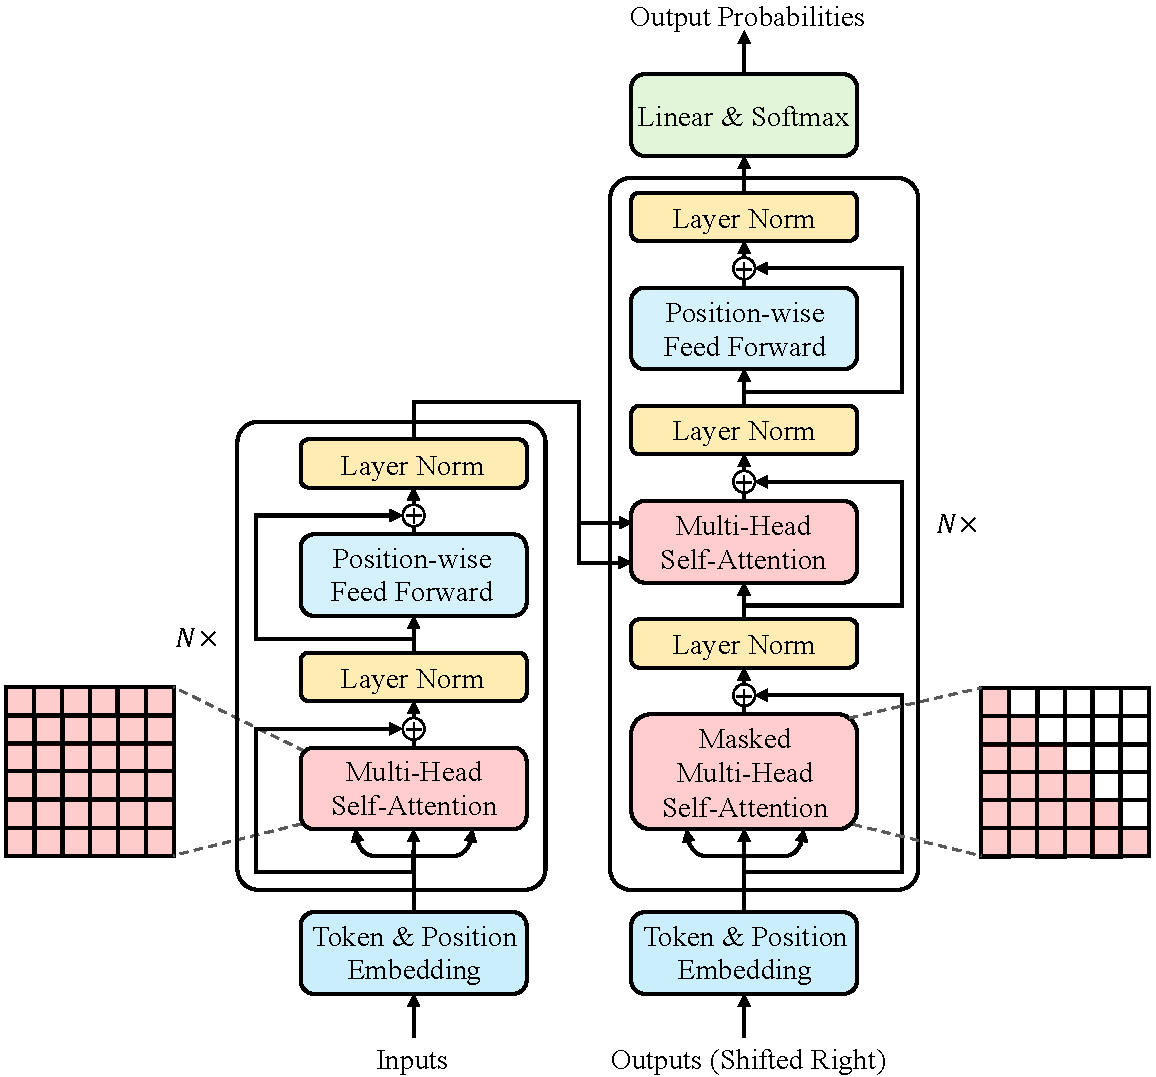
\includegraphics[width=0.65\linewidth]{images/Transformer_Encoder-Decoder_v2.pdf}}
    \hspace{0.2in}
    \subfigure[Decoder-only Models]{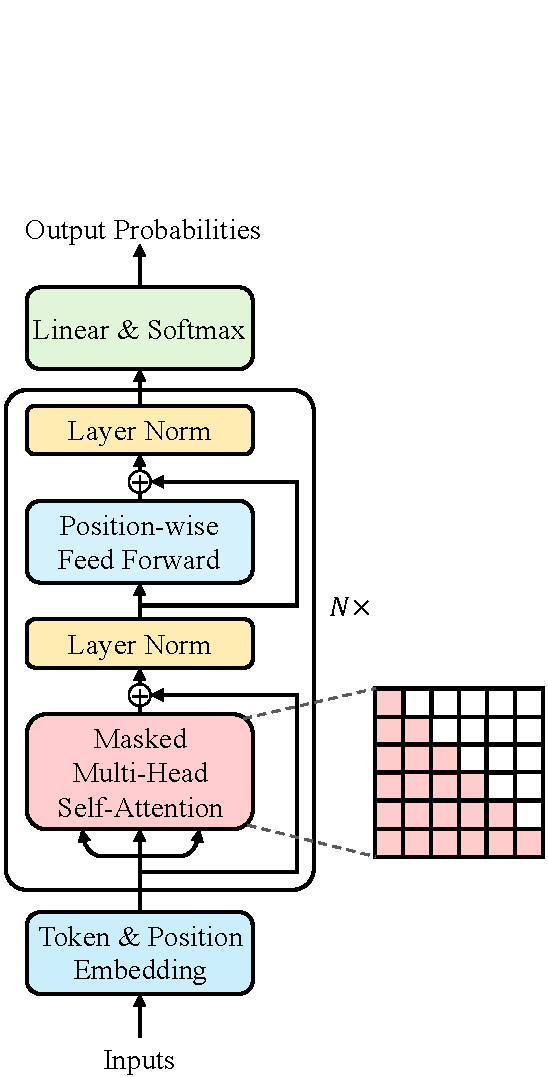
\includegraphics[width=0.3\linewidth]{images/Transformer_Decoder-Only_v2.pdf}}
\end{minipage}}
\caption{The overview of large language models (LLMs) with encoder-decoder and decoder-only Transformer architecture for code generation, adapted from \cite{vaswani2017attention}.}
\label{fig:architecture}   
\end{center}
\end{figure}
\subsubsection{Position-wise Feed-Forward Networks}
% In each Transformer layer, a Position-wise Feed-Forward Network (PFFN) is leveraged subsequent to the MHSA sub-layer to refine the sequence embeddings at each position $i$ separately and identically, encoding more intricate feature representations. 
% The PFFN is composed of a pair of linear transformations interspersed with a ReLU activation function. Formally,
Within each Transformer layer, a Position-wise Feed-Forward Network (PFFN) is leveraged following the MHSA sub-layer to refine the sequence embeddings at each position $i$ in a separate and identical manner, thereby encoding more intricate feature representations. 
The PFFN is composed of a pair of linear transformations, interspersed with a ReLU activation function. Formally,
\begin{equation}
\begin{aligned}
\operatorname{PFFN}(h^{(l)})=\left(\operatorname{Concat}\left\{\operatorname{FFN}(h^{(l)}_i)^T\right\}_{i=1}^{n}\right)^T,
\end{aligned}   
\end{equation}
\begin{equation}
\begin{aligned}
\operatorname{FFN}(h^{(l)}_i)=\operatorname{ReLU}(h^{(l)}_i\mathbf{W}^{(1)}+b^{(1)})\mathbf{W}^{(2)}+b^{(2)},
\end{aligned} 
\end{equation}
where $h^{(l)} \in \mathbb{R}^{n\times d_{model}}$ is the outputs of MHSA sub-layer in $l$-th Transformer layer, and $h^{(l)}_i \in \mathbb{R}^{d_{model}}$ denotes the latent representation at each sequence position. The projection matrices $\left\{\mathbf{W}^{(1)}, (\mathbf{W}^{(2)})^T \right\} \in \mathbb{R}^{d_{model} \times 4d_{model}}$ and bias vectors $\{\mathbf{b}^{(1)}, \mathbf{b}^{(2)}\} \in \mathbb{R}^{d_{model}}$ are parameters learned during training. These parameters remain consistent across all positions while are individually initialized from layer to layer. In this context, $T$ represents the transpose operation on a matrix.

\subsubsection{Residual Connection and Normalization}
% In order to alleviate the problem of gradients vanishing or exploding caused by network deepening, Transformer employs a residual connection \cite{he2016deep} around each abovementioned module, followed by Layer Normalization \cite{ba2016layer}. 
% For the placement of Layer Normalization operation, it has two widely used approaches:
% 1) \textbf{Post-Norm}: layer normalization is placed after the element-wise residual addition, following the vanilla Transformer \cite{vaswani2017attention}.
% 2) \textbf{Pre-Norm}: layer normalization is applied to the input of every sub-layer, such as GPT-2 \cite{radford2019language}. Formally, it can be formulated as: 
To alleviate the issue of vanishing or exploding gradients resulting from network deepening, the Transformer model incorporates a residual connection \cite{he2016deep} around each of the aforementioned modules, followed by Layer Normalization \cite{ba2016layer}. 
For the placement of Layer Normalization operation, there are two widely used approaches:
1) \textbf{Post-Norm}: Layer normalization is implemented subsequent to the element-wise residual addition, in accordance with the vanilla Transformer \cite{vaswani2017attention}.
2) \textbf{Pre-Norm}: Layer normalization is applied to the input of each sub-layer, as seen in models like GPT-2 \cite{radford2019language}. 
Formally, it can be formulated as:
\begin{equation}
\begin{aligned}
\textbf{Post-Norm}: 
    \mathbf{H^{(l)}} &=\operatorname{LayerNorm}(\operatorname{PFFN}(\mathbf{h^{(l)}})+\mathbf{h^{(l)}}),\\
    \mathbf{h^{(l)}}&=\operatorname{LayerNorm}(\operatorname{MHSA}(\mathbf{H^{(l-1)}})+\mathbf{H^{(l-1)}}) 
\end{aligned}
\end{equation}
\begin{equation}
\begin{aligned}
\textbf{Pre-Norm}: 
    \mathbf{H^{(l)}} &=\operatorname{PFFN}(\operatorname{LayerNorm}(\mathbf{h^{(l)}}))+\mathbf{h^{(l)}},\\
    \mathbf{h^{(l)}}&=\operatorname{MHSA}(\operatorname{LayerNorm}(\mathbf{H^{(l-1)}}))+\mathbf{H^{(l-1)}} 
\end{aligned}
\end{equation}
\subsubsection{Positional Encoding}
% As self-attention alone cannot capture the position information of each input token, the vanilla Transformer adds an absolute positional encoding approach to supplement positional information, which is known as sinusoidal position embeddings \cite{vaswani2017attention}. 
% Concretely, for token in position $pos$, the position embedding is defined as:
Given that self-attention alone cannot discern the positional information of each input token, the vanilla Transformer introduces an absolute positional encoding method to supplement this positional information, known as sinusoidal position embeddings \cite{vaswani2017attention}. 
Specifically, for a token at position $pos$, the position embedding is defined as:
\begin{equation}\label{eq:sin}
\begin{aligned}
    \mathbf{p}_{pos,2i}=\sin(\frac{pos}{10000^{2i/d_{model}}}),
\end{aligned}
\end{equation}
\begin{equation}\label{eq:cos}
\begin{aligned}
    \mathbf{p}_{pos,2i+1}=\cos(\frac{pos}{10000^{2i/d_{model}}}), 
\end{aligned}
\end{equation}
where $2i, 2i+1$ represent the dimensions of the position embedding, while $d_{model}$ denotes the model dimension. Subsequently, each position embedding is added to the corresponding token embedding, and the sum is fed into the Transformer. 
Since the inception of this method, a variety of innovative positional encoding approaches have emerged, such as learnable embeddings \cite{devlin2018bert}, relative position embeddings \cite{shaw2018self}, RoPE \cite{su2024roformer}, and ALiBi \cite{press2021train}. 
% The more details of each method refer to \cite{lin2022survey,zhao2023length}.
For more detailed descriptions of each method, please consult \cite{lin2022survey,zhao2023length}.

\subsubsection{\done{Architecture}}
\done{
There are two types of Transformer architecture for code generation task, including encoder-decoder and decoder-only. 
For the encoder-decoder architecture, it consists of both an encoder and a decoder, in which the encoder processes the input data and generates a set of representations, which are then used by the decoder to produce the output.
However, for decoder-only architecture, it consists only of the decoder part of the transformer, where it uses a single stack of layers to both process input data and generate output.
Therefore, the encoder-decoder architecture is suited for tasks requiring mapping between different input and output domains, while the decoder-only architecture is designed for tasks focused on sequence generation and continuation.
The overview of LLMs with these two architectures are illustrated in Figure \ref{fig:architecture}.
}


\subsection{Code Generation}
% Code generation refers to generating source code with LLM from natural language descriptions, a process also known as a natural-language-to-code task.
% Typically, the natural language descriptions contain programming problem descriptions (or docstring) and optionally some programming context (e.g., function signature, assertions, and so on). 
% Formally, the natural language (NL) descriptions can be denoted as $\mathbf{x}$. 
% Given $\mathbf{x}$, employing a LLM with model parameters $\theta$ to generate a code solution $\mathbf{y}$ can be denoted as $P_{\theta}(\mathbf{y}\mid\mathbf{x})$. 
% To verify the functionality correctness of code solution, code solution $\mathbf{y}$ is later executed via a compiler or interpreter, denoted as $\mathbf{Exe}(\cdot)$, on a suit of unit tests. The execution feedback can be represented by $\mathbf{Feedback}(\mathbf{Exe}(\mathbf{y}))$.
Large language models (LLMs) for code generation refer to the use of LLM to generate source code from natural language descriptions, a process also known as a natural-language-to-code task.
Typically, these natural language descriptions encompass programming problem statements (or docstrings) and may optionally include some programming context (e.g., function signatures, assertions, etc.). 
Formally, these natural language (NL) descriptions can be represented as $\mathbf{x}$.
Given $\mathbf{x}$, the use of an LLM with model parameters $\theta$ to generate a code solution $\mathbf{y}$ can be denoted as $P_{\theta}(\mathbf{y}\mid\mathbf{x})$.
% With the advent of in-context learning abilities of LLM \cite{wei2022emergent}, some exemplars are often postpended at natural language description $\mathbf{x}$ as the demonstrations to improve the performance of code generation or constrain the generation format, etc \cite{li2023towards,patel2023evaluating}. A fixed set of $M$ exemplars is denoted as $\{(\mathbf{x_i}, \mathbf{y_i})\}_{i=1}^M$. Therefore, following \cite{ni2023lever}, a more general formulation of LLMs for code generation with few(zero)-shot exemplars can be revised by:
The advent of in-context learning abilities in LLM \cite{wei2022emergent} has led to the appending of exemplars to the natural language description $\mathbf{x}$ as demonstrations to enhance code generation performance or constrain the generation format \cite{li2023towards,patel2023evaluating}. 
A fixed set of $M$ exemplars is denoted as $\{(\mathbf{x_i}, \mathbf{y_i})\}_{i=1}^M$. 
Consequently, following \cite{ni2023lever}, a more general formulation of LLMs for code generation with few-shot (or zero-shot) exemplars can be revised as:
\begin{equation}
\begin{aligned}
   P_\theta(\mathbf{y}\mid\mathbf{x}) \Rightarrow P_\theta(\mathbf{y}\mid\operatorname{prompt}(\mathbf{x}, \{(\mathbf{x_i}, \mathbf{y_i})\}_{i=1}^k)), k\in\{0, 1, \dots, M\}
\end{aligned}
\end{equation}
where $\operatorname{prompt}(\mathbf{x}, \{(\mathbf{x_i}, \mathbf{y_i})\}_{i=1}^k))$ is a string representation of the overall input, and $\{(\mathbf{x_i}, \mathbf{y_i})\}_{i=1}^k$ denotes a set of $k$ exemplars randomly selected from $\{(\mathbf{x_i}, \mathbf{y_i})\}_{i=1}^M$. 
In particular, when $k=0$, this denotes zero-shot code generation, equivalent to vanilla ones without in-context learning.  
\done{In the decoding process}, a variety of decoding strategies can be performed for code generation, including deterministic-based strategies (e.g., greedy search and beam search) and sampling-based strategies (e.g., temperature sampling, top-k sampling, and top-p (nucleus) sampling). 
% The details of each decoding strategy refer to \cite{holtzman2019curious}. 
For more detailed descriptions of each decoding strategy, please consult \cite{holtzman2019curious}. \done{For example, the greedy search and sampling-based decoding strategies can be formulated as follows:}
\begin{equation}
\begin{aligned}
\textbf{Greedy Search}:
   \mathbf{y^*} = \mathop{\mathrm{argmax}}_\mathbf{y} P_\theta(\mathbf{y}\mid\operatorname{prompt}(\mathbf{x}, \{(\mathbf{x_i}, \mathbf{y_i})\}_{i=1}^k)), k\in\{0, 1, \dots, M\}
\end{aligned}
\end{equation}
\begin{equation}
\begin{aligned}
\textbf{Sampling}: 
   \mathbf{y} \sim P_\theta(\mathbf{y}\mid\operatorname{prompt}(\mathbf{x}, \{(\mathbf{x_i}, \mathbf{y}_i)\}_{i=1}^k)), k\in\{0, 1, \dots, M\}
\end{aligned}
\end{equation}

\done{To verify the functionality correctness of the generated code solution, $\mathbf{y}$ is subsequently executed via a compiler or interpreter, represented as $\mathbf{Exe}(\cdot)$, on a suit of unit tests $\mathbf{\mathcal{T}}$. 
The feedback from this execution can be denoted as $\mathbf{Feedback}(\mathbf{Exe}(\mathbf{y},\mathbf{\mathcal{T}}))$. 
If the generated code solution fails to pass all test cases, the error feedback can be iteratively utilized to refine the code by leveraging the previous attempt ($\mathbf{y}_{pre}$) and the associated feedback. Formally,
\begin{equation}
\begin{aligned}
    \mathbf{y} \sim P_\theta(\mathbf{y}\mid\operatorname{prompt}(\mathbf{x}, \{(\mathbf{x_i}, \mathbf{y_i})\}_{i=1}^k, \mathbf{y}_{pre}, \mathbf{Feedback}(\mathbf{Exe}(\mathbf{y},\mathbf{\mathcal{T}})))), k\in\{0, 1, \dots, M\}
\end{aligned}
\end{equation}
Further details and relevant studies on using feedback to improve code generation are comprehensively discussed in Section \ref{sec:reinforcement_learning} and \ref{sec:prompting}.
}


